\chapter{Priporočilni sistemi}

Priporočilni sistemi so danes v računalništvu in informatiki prisotni
praktično povsod. Še najbolj očitno se z njimi srečamo pri obisku
raznih spletnih strani, kot so Facebook, eBay, Amazon, IMDB, Netflix in podobnih. Te strani si vneto beležijo podatke o naših obiskih, ogledu izbranih podstrani, kupljenih izdelkih, ki jih strani ponujajo, ali pa odzivih na ponujene informacije (so nam te všeč ali ne?). Samo na podlagih naših podatkov bi te strani ne bile preveč ``pametne''. A ker se tam zbirajo podatki tudi o vseh ostalih obiskovalcih, je lahko na ta način zbranih informacij hitro dovolj. ``Inteligenco'' te strani kažejo v vsebinah, ki so prilagojene nam, uporabnikom. Strani nam svetujejo, kaj vse bi se nam splačalo pogledati, katere izdelke ali druge strani bi lahko bile zanimive in kaj nasploh lahko še počnemo glede na naše, največkrat implicitno izražene interese.

Jedro takih spletnih strani, programov in sistemov so priporočilni sistemi. Ti
lahko na podlagi zbranih informacij o uporabnikih sklepajo o uporabnikovih preferencah, željah in interesih. Za posameznega uporabnika lahko recimo na podlagi njemu podobnih uporabnikov napovedo, kaj bi uporabnika lahko (še) zanimalo in mu ponudijo ogled stvari, ki jih ta do sedaj še ni pogledal, pa bi ga morda lahko navdušile. Uporabnost in privlačnost teh priporočilnih storitev ter posledično njihova finančna uspešnost je lahko zelo odvisna od kvalitete uporabljenih priporočilnih sistemov oziroma temu, kako dobro ti modelirajo dejanske uporabnikove interese.

Priporočilni sistemi so lahko uporabni v trženju, analitiki in priporočanju v socialnih omrežjih, biomedicini, humanistiki, astronomiji, kemiji -- pravzaprav jih lahko uporabimo prav na vseh področjih, kjer se zbirajo podatki o uporabnikih in stvareh, ki jih neka spletna stran ali programskih sistem, ali pa dejanska fizična trgovina ponuja. V tem poglavju se bomo osredotočili na priporočilne sisteme, ki delujejo na preferencah, ki so jih uporabniki eksplicitno ali implicitno podali o množici stvari. Ko govorimo o ``stvareh'' mislimo na izdelke, spletne strani, filme, glasbo, kakršnekoli koncepte, torej na karkoli, o čemer so se uporabniki preko neke storitve ali spletne strani izrekli. Stvari so uporabniku lahko bile všeč ali ne, lahko jih je številčno ocenil, morda samo označil zanimive izdelke. Lahko pa si je sistem samo zapomnil, katere spletne strani ali storitve je uporabnik izbral, katero glasbo je poslušal ali kateri film si je ogledal. Vrsto priporočilnih sistemov, ki temelji na takem preferenčnem znanju in pri podajanju priporočil uporablja uporabniške profile vseh ostalih uporabnikov v sistemu imenujemo skupinsko filtriranje \angl{collaborative filtering}.

Čeprav bomo v tem poglavju govorili samo o skupinskem filtriranju, naj
tu omenimo, da obstajajo tudi drugačni pristopi k priporočanju. Na
spletu recimo lahko najdemo sezname najboljših izdelkov določenega
tipa, ki jih je priporočil nek urednik ali pisatelj bloga. Spletne
strani, kot so na primer domača enaa.com, nam na vhodni strani
predlaga izdelke, ki so najbrž izbrani med najbolj dostopanimi ali pa
so bili v preteklem obdobju s strani vseh uporabnikov najbolje
ocenjeni. Tu gre za enostavno združevanje ocen uporabnikov, ali pa
uporabo enostavnih postopkov štetja dostopov uporabnikov do izdelkov.

Uporabimo lahko tudi dodatna znanja o uporabnikih in stvareh. Uporabnike lahko opišemo s starostjo, spolom, naštejmo interesna področja, ki jih zanimajo, opišemo, kaj delajo v službi, kakšni so njihovi hobiji, ali pa celo s kom se družijo. Stvarem lahko določimo njihov namen, jih opremimo s ključnimi besedami iz opisa, razvrstimo v razne skupine. Na podlagi teh podatkov lahko priporočilni sistemi sklepajo o nam podobnih uporabnikih ali pa stvareh, ki so podobne tem, ki smo jih že pozitivno ocenili. Priporočilne sisteme, ki temeljijo na takem dodatnem poznavanju uporabnikov in stvari \angl{knowledge-based recommendation systems} je morda, zaradi potrebnih dodatnih podatkov, je tipično težje vzpostaviti od sistemov skupinskega filtriranja, njihova točnost pa je presenetljivo lahko celo slabša od točnosti slednjih. Uporaba metod, ki uporabljajo dodatna znanja o uporabnikih in stvareh, je lahko ključna pri hladnem zagonu sistema \angl{cold start}, ko uporabnik storitve še ni uporabljal in zanj še nimamo nimamo podatkov o preferencah oziroma všečnosti stvari, na katerih bi temeljila priporočila skupinskega filtriranja.

V nadaljevanju spregovorimo torej samo o tehnikah skupinskega filtriranja. Priporočilnim sistemom, ki uporabljajo dodatna znanja, se izognemo, bo pa radovedni bralec lahko sam razpoznal, da bi bilo moč te tehnike enostavno razviti in pri tem uporabiti zelo podobne koncepte kot pri skupinskem filtriranju. Oba pristopa namreč temeljita na ocenjevanju podobnosti med uporabniki in med stvarmi, razlikujeta se le v načinu, kako te podobnosti izračunamo in v podatkih, ki jih za to uporabimo.

\section{Podatki}

Naš cilj je razviti priporočilni sistem za skupino uporabnikov $\mathcal{U}$, ki lahko izbirajo med množico stvari $\mathcal{I}$, kjer bomo imeli $N$ različnih uporabnikov ($|\mathcal{U}|=N$) in $M$ različnih stvari ($\mathcal{I}=M$). Preferenčno znanje $\mathcal{R}$ bomo zapisali kot množico trojk $(u,i,r)$ za uporabnika $u\in\mathcal{U}$, stvar $i\in\mathcal{I}$ in preferenco $r$, ki bo podala oceno oziroma zaželenosti stvari $i$ s strani uporabnika $u$.

Preference merimo v neki izbrani merski lestvici. Na primer, ocene zapišemo s celimi števili od 1 do 5, ali pa od 0 do 10, ali pa z realnimi števili od 0.0 do 1.0 ali pa od -1.0 do 1.0. Včasih pa imamo na voljo samo oznake, ali je uporabnik za določeno stvar izrazil zanimanje. Slednji primer je težji, saj nimamo urejenih ocen oziroma imamo samo označene pozitivne preference. Predpostavka, da so vse stvari, ki jih uporabnik ni označil, zanj nezanimive, pa je lahko napačna. V tem poglavju se bomo predvsem ukvarjali s podatki, kjer imamo na voljo numerične ocene, tu in tam pa bomo namignili, kako bi lahko obravnavali podatki, ki vsebujejo samo seznam zanimivih stvari, za katere uporabnik ni podal preferenčne ocene v neki numerični lestvici.

Priporočilne sisteme lahko razvijamo za manjše skupine uporabnikov in stvari, opravka pa imamo lahko tudi z večjimi množicami, kjer je lahko število uporabnikov in stvari tudi po več tisoč, sto tisoč ali pa celo nekaj milijonov. Celotno preferenčno znanje, torej ocene za vse kombinacije uporabnikov in stvari tako ne bo nikoli dostopno, opravka pa bomo imeli samo z manjšim vzorcem preferenčnega znanja, ki ga označimo s $\tau'\subset\mathcal{R}$. Ker bomo na podlagi tega vzorca zgradili naš priporočilni sistem, ga tu imenujmo učna množica. Predpostavili bomo, da obstaja največ ena ocena za vsako kombinacijo $(u, i)$, torej kombinacijo uporabnik-stvar. Ker se bomo še največkrat spraševali o tem, ali naša učna množica vsebuje oceno za dan par $(u,i)$, uvedimo množico parov $\tau$, za katere imamo dano preferenčno znanje:
%
$$\tau=\{(u,i); \exists r:(u,i,r)\in\tau'\}$$
%
Preferenčno oceno uporabnika $u$ za stvar $i$ zapišimo z $r_{u,i}$. Množica ocen izbranega uporabnika $u$ tvori uporabniški profil ${\bf r}_u$. Podobno lahko vse ocene uporabnikov za izbrano stvar $i$ zberemo v stvarni profil oziroma profil stvari ${\bf r}_i$.

Primer s seznamom podanega preferenčnega znanja podaja tabela~\ref{t:pref-ocene}, kjer so
\begin{eqnarray}
{\mathcal U} & = & \{ {\rm Mojca}, {\rm Miha}, {\rm Sandra}, {\rm Jana}, {\rm Tina}, {\rm Nik}, {\rm Janez}, {\rm Cene} \} \nonumber \\
{\mathcal I} & = & \{ {\rm olive}, {\rm vampi}, {\rm testenine}, {\rm blitva}, {\rm ocvirki}, {\rm krofi} \} \nonumber
\end{eqnarray}

\begin{table}
\caption{Primer preferenčnega znanja podanega kot množica trojk (uporabnik, stvar, ocena).}
\label{t:pref-ocene}
\begin{center}
\small
\begin{tabular}{lll}
\toprule
uporabnik & izdelek & ocena \\
\midrule
Mojca & olive & 5.0 \\
Mojca & vampi & 1.2 \\
Mojca & testenine & 4.1 \\
Mojca & blitva & 5.0 \\
Miha & ocvirki & 4.3 \\
Miha & vampi & 4.9 \\
Miha & blitva & 1.2 \\
Sandra & ocvirki & 2.3 \\
Sandra & olive & 5.0 \\
Sandra & vampi & 0.1 \\
Sandra & blitva & 5.0 \\
Jana & ocvirki & 4.0 \\
Jana & vampi & 3.0 \\
Jana & krofi & 4.5 \\
Tina & olive & 5.0 \\
Tina & krofi & 3.5 \\
Tina & testenine & 2.1 \\
Tina & blitva & 4.6 \\
Nik & ocvirki & 2.0 \\
Nik & olive & 3.8 \\
Nik & vampi & 0.3 \\
Janez & olive & 0.3 \\
Janez & vampi & 4.8 \\
Janez & testenine & 2.5 \\
Cene & ocvirki & 3.9 \\
Cene & krofi & 4.8 \\
Cene & blitva & 3.0 \\
\bottomrule
\end{tabular}
\end{center}
\end{table}

Namesto podajanja preferenčnega znanja oziroma naše učne množice s trojkami (uporabnik, stvar, ocena) bi lahko, konceptualno, to znanje zapisali v obliki matrike (tabela~\ref{t:pref-matrika}). ``Konceptualno'' namreč zato, ker bi za večjo skupino uporabnikov in stvari take matrike postale izjemno velike in ker jih kot take, v resnih računalniških implementacijah, nikoli eksplicitno ne uporabimo, ampak namesto njih podatke zapišemo v slovarje.

\begin{table}
\caption{Primer preferenčnega znanja podanega z matriko}
\label{t:pref-matrika}
\begin{center}
\begin{tabular}{lcccccc}
\toprule
& olive & vampi & testenine & blitva & ocvirki & krofi \\
\midrule
Mojca & 5.0 & 1.2 & 4.1 & 5.0 & & \\
Miha & 4.3 & 4.9 & & 1.2 & & \\
Sandra & 5.0 & 0.1 & & 5.0 & 2.3 & \\
Jana & & 3.0 & & & 3.0 & 4.5 \\
Tina & 5.0 & & 2.1 & 4.6 & & 3.5 \\
Nik & 3.8 & & & & 2.0 & \\
Janez & 0.3 & 4.8 & 2.5 & & & \\
Cene & & & & 3.0 & 3.9 & 4.8 \\
\bottomrule
\end{tabular}
\end{center}
\end{table}

\section{Skupinsko filtriranje na podlagi podobnosti}

Skupinsko filtriranje \angl{collaborative filtering} je danes ena od osnovnih, morda glavnih tehnik za izdelavo praktičnih priporočilnih sistemov, ki temeljijo na preferenčnem znanju množic uporabnikov. Za danega uporabnika v teh sistemih predpostavimo, da je ta že ocenil določene stvari. Priporočilo, katera stvar ga bi zanimala med temi, za katere še ni podal preference, pridobimo tako, da za vse take stvari izračunamo pripadajočo oceno (preferenco) ter uporabniku priporočimo stvar, ki je bila na ta način najbolje ocenjena. Priporočila za danega uporabnika razvijemo ob predpostavki, da je v celotni množici uporabnikov nekaj takih, ki so izbranemu uporabniku podobni. Stvari, ki so všeč njim, bodo najbrž všeč tudi izbranemu uporabniku. 

Najbolj neposreden način, ki se ga pri napovedovanju ocen lahko poslužimo je, da na podlagi že danih ocen izračunamo, kako podobni so med seboj uporabniki ter ocene ostalih uporabnikov za posamezno stvar utežimo s podobnostjo ciljnemu uporabniku. 

\subsection{Podobnost med uporabniki}

Za danega uporabnika $u$ nas zanima, kako podobni so mu ostali uporabniki. Določiti moramo mero podobnosti med uporabniškimi profili. Spomnimo se: uporabniški profil je množica vseh ocen stvari, ki jih je uporabnik ocenil oziroma za katere imamo podatke v učni množici. Nekaj kandidatov za mere podobnosti poznamo že iz prejšnjih poglavij, zato tu le na hitro omenimo, da je primerna in mnogokrat uporabljana mera kosinusne podobnosti:
%
$$ s_{\rm c}(u,u')={{\bf r}_u {\bf r}_{u'} \over |{\bf r}_u|\ |{\bf r}_{u'}|}$$
%

Pri kosinusni podobnosti v skalarnem produktu manjkajoče podatke izpustimo. Ko računamo razdaljo med Mojco in Mihom, na primer, bomo upoštevali samo ocene za olive, vampe in blitvo. Njuna profila za te tri stvari bosta zato $(5.0, 1.2, 5.0)$ in $(4.3, 4.9, 1.2)$. Skalarni produkt teh dveh vektorjev znaša $33.38$. Pri računanju dolžine pa upoštevamo celoten Mojčin in Mihov profil. Dolžini njunih profilov sta tako $8.26$ in $6.63$, torej je njuna kosinusna podobnost enaka $0.61$. Podobnost med Mojco in Tino (vektorja, ki ju primerjamo, sta $(5.0, 4.1, 5.0)$ in $(5.0, 2.1, 4.6)$) je večja in znaša $0.86$. Opazimo tudi lahko, da bo recimo podobnost med Janezom in Cenetom enaka $0.0$, saj ne obstaja izdelek, ki bi ga ta dva uporabnika oba ocenila.

V primeru, da preferenčnih ocen nimamo in uporabniške profile tvori samo seznam stvari, ki so uporabniku všeč, lahko oceno podobnosti med uporabniki izračunamo z mero po Jaccardu:
%
$$ s_{\rm J}(u, u')={||{\bf r}_u\cap{\bf r}_{u'}|| \over ||{\bf r}_u\cup{\bf r}_{u'}||}$$
kjer smo, na primer, z $||{\bf r}_u\cap{\bf r}_{u'}||$ označili število stvari, ki so všeč tako uporabniku $u$ kot uporabniku $u'$.

\subsection{Priporočila na podlagi uporabniških profilov in podobnosti med uporabniki}

Za danega uporabnika $u$ želimo z uporabo učnih podatkov oceniti, kakšna je njegova preferenčna ocena za stvar $i$. To označimo z $\hat{r}_{ui}$, saj gre za oceno oziroma približek. Preferenčno oceno lahko na ta način pridobimo tudi za že obstoječo oceno iz učne množice, a bo ta verjetno različna od ocene $r_{ui}$, ki jo je podal uporabnik in bomo pri njeni napovedi storili določeno napako.

Izhodišče za izračun preference $\hat{r}_{ui}$, torej ocene koristnosti stvari $i$ za uporabnika $u$, so podobnosti med uporabniki. Ideja pa je enostavna: pogledamo, kdo so vsi uporabniki, ki so ocenili stvar $i$. Njihove ocene utežimo s podobnostjo s ciljnim uporabnikom $u$ ter dobljeno vsoto normiramo z vsoto uteži:

\begin{equation}
\hat{r}_{ui} = \frac{\displaystyle\sum_{u':(u',i)\in\tau,\ u'\neq u}s(u,
  u')\times r_{u'i}}{\displaystyle\sum_{u':(u',i)\in\tau,\ u'\neq u}s(u, u')}
\end{equation}

\subsection{Priporočila na podlagi profilov stvari in podobnosti med stvarmi}

Tudi stvari imajo svoje profile. Če so uporabniški profili vrstični vektorji v preferenčni matriki, katere primer je prikazan v tabeli~\ref{t:pref-matrika}, so profili stvari stolpci te matrike, oziroma stolpčni vektorji. Za stvar $i$ njen profil zapišemo z ${\bf r}_i$. Podobno kot za dva uporabnika lahko podobnost med stvarmi merimo, na primer s kosinusno razdaljo:
%
$$ s_{\rm c}(i,i')={{\bf r}_i {\bf r}_{i'} \over |{\bf r}_i|\ |{\bf r}_{i'}|}$$
%

Sedaj pa nazaj k priporočanju. Želeli bi torej oceniti preferenco $\hat{r}_{ui}$, ki jo ima za stvar $i$ uporabnik $u$. Predpostavljamo, da je uporabnik že ocenil nekaj drugih stvari (vsako od teh bomo označili z $i'$). Oceno za stvar $i$ lahko izračunamo iz teh ocen, a pri tem močneje upoštevamo tiste stvari, ki so podobne stvari $i$, ki jo ocenjujemo:
%
\begin{equation}
\hat{r}_{ui} = \frac{\displaystyle\sum_{i':(u,i')\in\tau,\ i'\neq i}s(i,
  i')\times r_{ui'}}{\displaystyle\sum_{i':(u,i')\in\tau,\ i'\neq i}s(i, i')}
\end{equation}

Ta izračun je na moč podoben izračunu iz prejšnjega razdelka, le da tu utežimo ocene našega ciljnega uporabnika, v prejšnjem razdelku pa smo utežili ocene ostalih uporabnikov.

\subsection{Priporočanje na podlagi podobnosti uporabnikov in stvari}

Priporočilno tehniko iz prejšnjih dveh podpoglavij lahko združimo. Iz učne množice lahko vzamemo poljubno oceno $r_{u'i'}$ ter jo utežimo glede na podobnost s ciljnim uporabnikom $u$ in ciljno stvarjo $i$, za katero oceno $\hat{r}_{ui}$ iščemo. Utežena vsota vseh teh ocen je naš približek za $\hat{r}_{ui}$:
%
\begin{equation}
\hat{r}_{ui} = \frac{\displaystyle\sum_{(u',i')\in\tau,\ (u',i')\neq (u,i)}s(u,u')\times s(i, i')\times r_{u'i'}}{\displaystyle\sum_{(u',i')\in\tau,\ (u',i')\neq (u,i)}s(u,u')\times s(i, i')}
\end{equation}

Na prvi pogled se nam taka rešitev lahko zazdi še najboljša, oziroma bolj primerna od teh, ki smo jih omenjali v prejšnjih dveh podpoglavjih. A njena očitna slabost je časovna kompleksnost, saj moramo poznati praktično vse pare podobnosti, torej med ciljnim in vsemi ostalimi uporabniki in ciljno in vsemi ostalimi stvarmi. V prejšnjih dveh podpoglavjih smo namreč računali na to, da so ciljno stvar $i$ ocenili samo nekateri uporabniki in je bilo potrebno izračunati podobnosti samo za te. Oziroma, računali smo, da je uporabnik $u$ ocenil samo manjši nabor stvari in da je samo te potrebno primerjati s ciljno stvarjo $i$.

\subsection{Priporočanje kar tako}

Vrednost $\hat{r}_{ui}$ lahko ocenimo kar s povprečno oceno stvari $i$ vseh (ostalih) uporabnikov, ki so to stvar ocenili:
%
\begin{equation}
\hat{r}_{ui} = \frac{\displaystyle\sum_{(u',i)\in\tau,\ u'\neq u} r_{u'i}}{|\{(u',i)\in\tau,\ i'\neq i \}|}
\end{equation}
%
Ta ocena bo neodvisna od uporabnika, nam pa lahko služi za primerjavo z ostalimi načini izračuna $\hat{r}_{ui}$, kot smo jih podali zgoraj. To oceno lahko morda še dodatno popravimo tako, da upoštevamo povprečno oceno uporabnika:
%
\begin{equation}
\hat{r}_{ui} = {1\over 2}\frac{\displaystyle\sum_{(u',i)\in\tau,\ u'\neq u} r_{u'i}}{|\{(u',i)\in\tau,\ i'\neq i \}|} + {1\over 2}\frac{\displaystyle\sum_{(u,i')\in\tau,\ i'\neq i} r_{ui'}}{|\{(u,i')\in\tau,\ i'\neq i \}|}
\end{equation}
%

\section{Pristranost}

Uporabniki smo v naših ocenah pristrani: nekateri uporabniki bolj
vedre narave bodo stvari ocenjevali z višjimi ocenami, nekateri
uporabniki pa bodo le stežka dajali najvišje ocene. Problemu
pristranosti uporabnikov se lahko vsaj deloma izognemo tako, da vsem
ocenam iz učne množice odštejemo povprečno oceno uporabnika. Se pravi
$r_{ui}$ nadomestimo z $r_{ui}-\overline{{\bf r}_u}$. Tako
popravljene ocene potem uporabimo pri učenju. Pri napovedovanju pa ne
smemo pozabiti, da smo povprečne ocene uporabnika pred tem odšteli, in
zato za par $(u,i)$ napovemo preferenčno oceno z
$\hat{r}_{ui}+\overline{{\bf r}_u}$.

\section{Ocenjevanje kvalitete priporočilnih sistemov}

Tudi tu lahko uporabimo prečno preverjanje, ki ga tokrat izvedemo kar nad množico trojk $(u,i,r_{ui})$. Torej tako, kot če bi vzorec iz tabele~\ref{t:pref-ocene} vzeli za učenje, na preostalem delu pa preverili naše izračunane preferenčne ocene. Za ocenjevanje kvalitete priporočanja lahko uporabimo iste mere, kot smo jih uporabili pri regresiji, torej na primer RMSE ali pa $R^2$.

\section{Priporočanje z matričnim razcepom}

V tabeli~\ref{t:pref-matrika} smo učne podatke predstavili kot matriko R, katere elementi so ocene $r_{ui}$ uporabnika $u$ za stvar $i$. Matrika R je redka, za njo pa mora priporočilni sistem znati oceniti vrednost manjkajočih elementov. Ker je uporabnikov $N$, stvari pa $M$, je matrika R oblike $M\times N$.Tipično sta dimenziji $M$ in $N$ visoki: uporabnikov je lahko nekaj tisoč, deset tisoč ali celo milijon, stvari pa ravno tako.

Že iz poglavja o gručenju vemo, da lahko stvari in uporabnike razvrstimo v skupine in za te potem poiščemo tipične stvari in tipične uporabnike. Na primer, pri izposoji filmov bi lahko zaznali, da obstajajo uporabniki storitve, ki radi gledajo večinoma akcijske filme, pa uporabniki, ki gledajo samo filme, ki so narejeni v Hollywoodu ter uporabniki, ki jim to ne pade na misel in si sposojajo samo umetniške filme iz manjših produkcijskih hiš. Uporabnike bi zato lahko predstavili s kratkimi profili, ki bi nam poročali o zaželenosti posameznih filmskih zvrsti. Pravimo, da bi na ta način uporabnike opisali v latentnem prostoru filmov, torej v prostoru filmskih kategorij, ki jih moramo iz podatkov šele razbrati. Po drugi strani pa bi tudi filme lahko opisali s profili v latentnem prostoru skupin uporabnikov, torej skupin, ki jih prav tako moramo šele pridobiti. Ta opis, predstavitev podatkov v latentnem, navideznem prostoru skupin stvari in skupin uporabnikov lahko pridobimo z enotnim postopkom, ki mu pravimo matrični razcep.

V pristopu z matričnim razcepom matriko ${\rm R}_{N\times M}$ predstavimo z matrikami ${\rm P}_{N\times K}$ in ${\rm Q}_{K\times M}$ tako, da velja ${\rm R}\approx {\rm P}{\rm Q}$ in da je $K<<M, N$ (slika~\ref{f:matricni-razcep}). Torej, tako, da je produkt matrik ${\rm P}$ in ${\rm Q}$ po elementih čim bolj podoben prvotni matriki ${\rm R}$ oziroma elementom, ki so tam definirani. Konstanta $K$ podaja število latentnih dimenzij, in je pri obliki razcepa, kot smo ga določili tu, enaka tako za uporabnike kot za stvari. Pravimo ji tudi stopnja razcepa. Ker je $K$ veliko manjši od dimenzij $M$ in $N$, v skrajnem primeru pa enak 1, pomeni, da s produktom ${\rm P} {\rm Q}$ prav gotovo ne bomo mogli verno predstaviti matriko $\rm R$, torej tako, da bi vsi elementi produkta bili enaki elementom vhodne matrike $\rm R$ (torej, ${\rm P}{\rm Q}\equiv {\rm R}$).

\begin{figure}[htbp]
\begin{center}
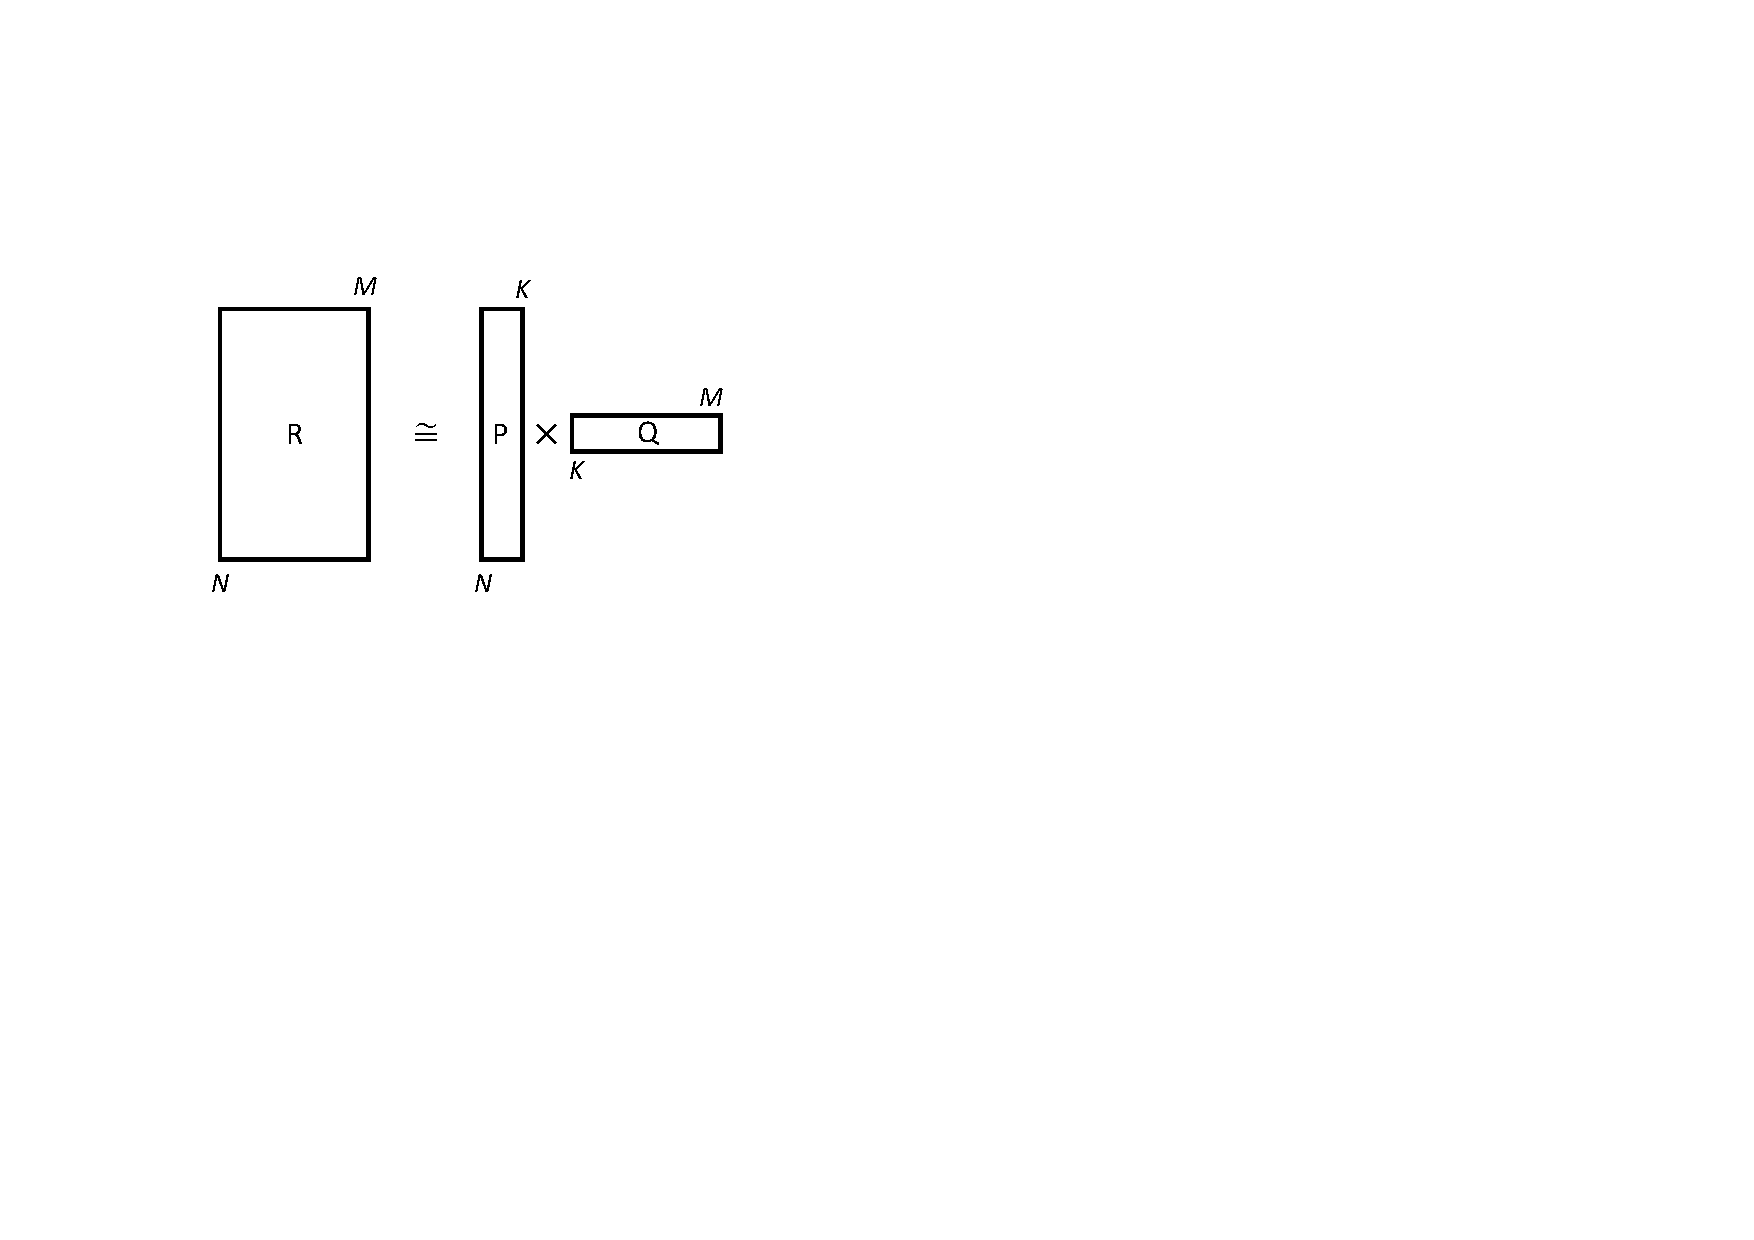
\includegraphics[width=7cm]{slike/matricni-razcep.pdf}
\caption{Razcep matrike R na manjši matriki P in Q.}
\label{f:matricni-razcep}
\end{center}
\end{figure}

Matrika $\rm P$ je matrika uporabniških profilov v latentnem prostoru filmov, torej prostoru tipičnih zvrsti filmov (teh nimamo, a jih pridobimo z razcepom matrike na produkt dveh matrik). Latentni profil uporabnika $u$ označimo z vektorjem ${\bf p}_u$. Podobno je matrika $\rm Q$ matrika profilov stvari v prostoru latentnih uporabnikov, profil stvari $i$ v tem prostoru pa zapišimo z vektorjem ${\bf q}_i$. Produkt latentnih profilov ustreza približku vrednosti ocene stvari $i$ uporabnika $u$, torej $\hat{r}_{ui}$ (slika~\ref{f:latentni-faktorji}).

\begin{figure}[htbp]
\begin{center}
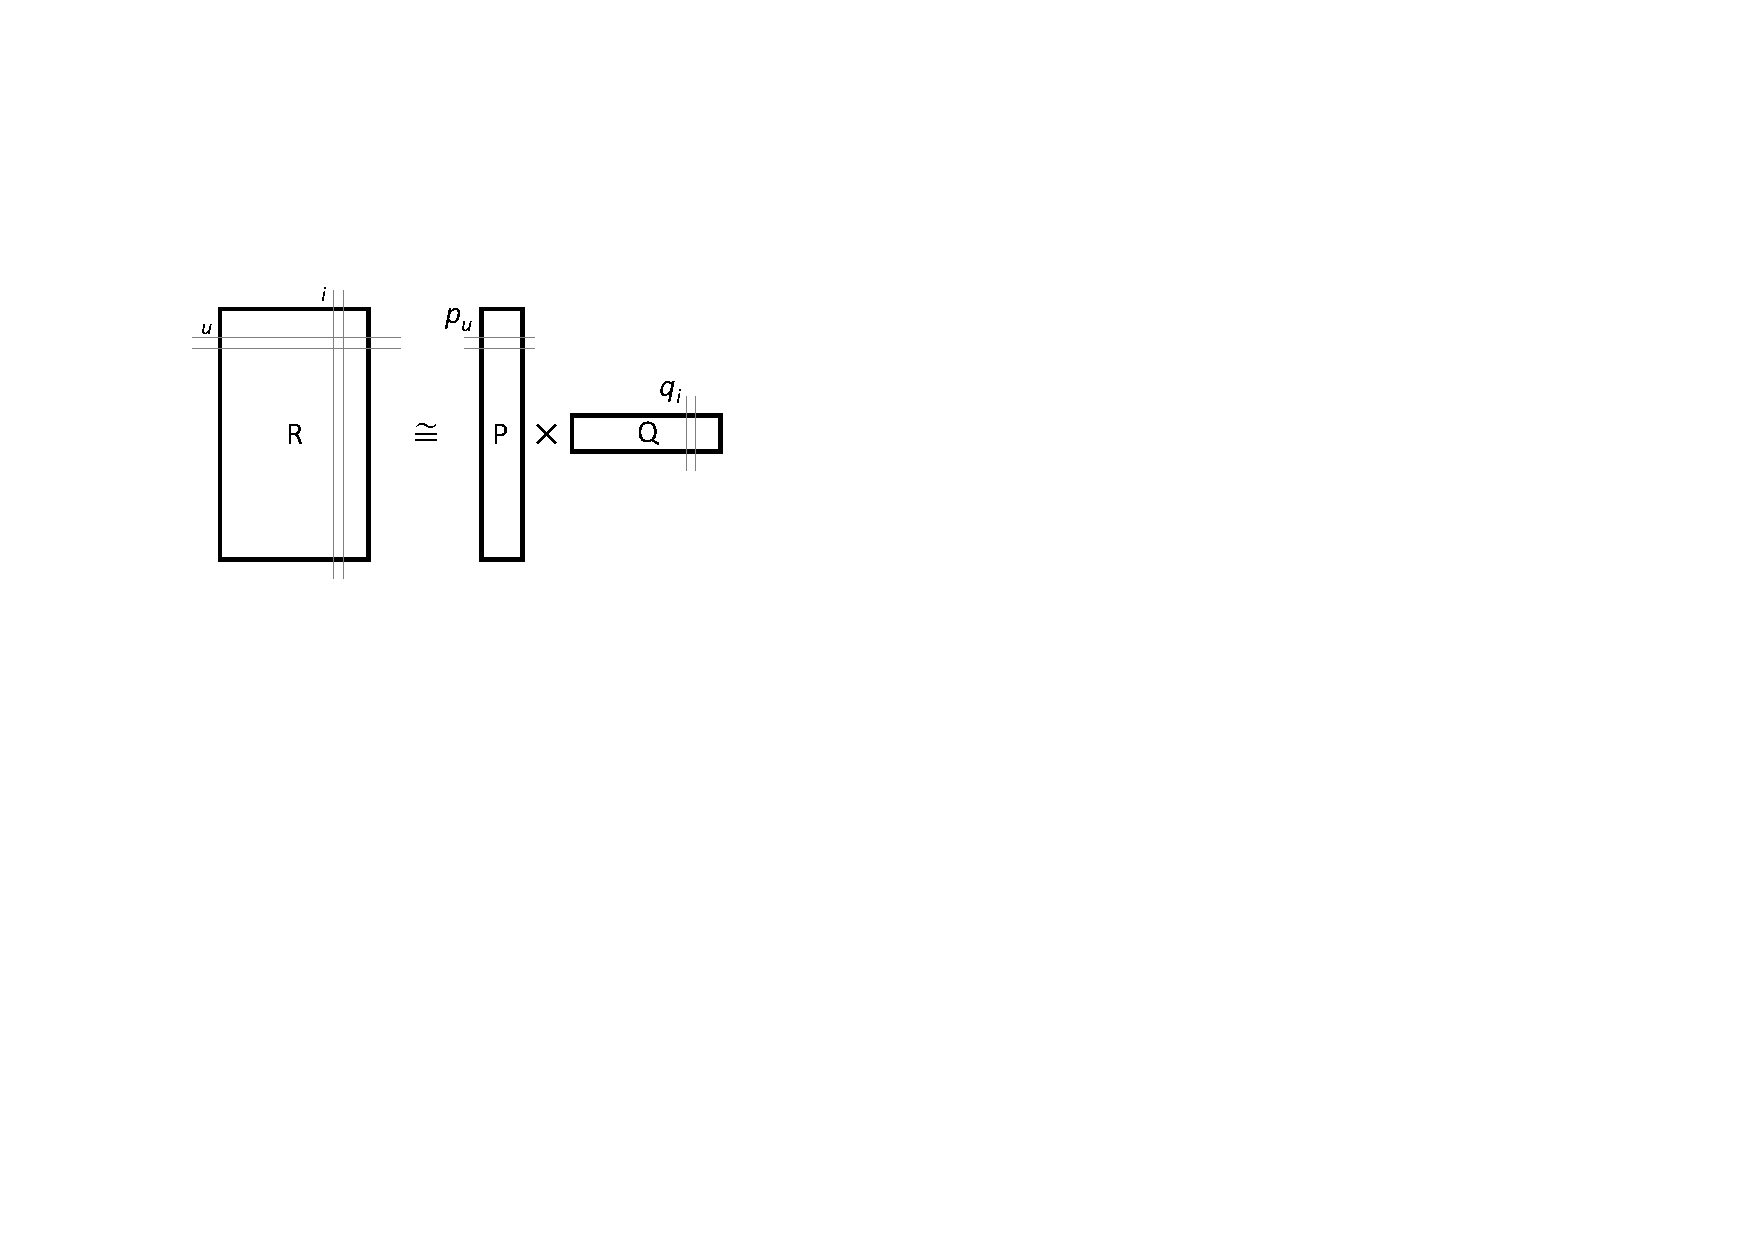
\includegraphics[width=7cm]{slike/latentni-faktorji.pdf}
\caption{Predstavitev uporabnika $u$ z latetnim profilom ${\bf p}_u$ in stvari $i$ z latentnim profilom ${\bf q}_i$. Skalarni produkt latentnih profilov nam da približek za oceno stvari $i$ uporabnika $u$, torej $\hat{r}_{ui}={\bf p}_u^T {\bf q}_i$.}
\label{f:latentni-faktorji}
\end{center}
\end{figure}

Razcep matrike R na matriki P in Q bomo poiskali tako, da bosta matriki P in Q polni, torej, da bodo vse vrednosti teh dveh matrik določene. Prav zato bomo lahko s produktom latentnih profilov lahko poiskali vrednost $\hat{r}_{ui}$ za vsako kombinacijo uporabnika $u$ in stvari $i$. Ostane nam torej le še, da izračunamo razcep, oziroma določimo matriki P in Q.

\subsection{Matrični razcep}

Z matrikami P in Q lahko izračunamo približek ocene za stvar $i$ uporabnika $u$, ki je:
%
\begin{equation}\label{eq:rui-latent}
  \hat{r}_{ui}={\bf p}_u^T {\bf q}_i = \sum_{k=1}^K p_{uk} q_{ki}
\end{equation}

Za ocene iz učne množice $r_{ui}$ bi želeli, da je ta približek čim boljši, oziroma da je napaka, ki jo s tem približkom naredimo, čim manjša. Izračunajmo kvadrat napake za oceno stvari $i$ uporabnika $u$:
%
\begin{equation}\label{eq:fact-error}
  e_{ui}^2 = (r_{ui}-\hat{r}_{ui})^2
\end{equation}
%
Želeli bi poiskati taki matriki $P$ in $Q$, kjer so te napake čim manjše. Ker bomo pri numeričnem iskanju teh matrik v vsaki iteraciji obravnavali natančno enega med učnimi primeri (torej $r_{ui}$ za določen par $(u,i)\in\tau$), potrebujemo izračunati gradient napake za vsakega od parametrov modela. Naš model sta matriki P in Q, vrednosti parametrov modela pa vsi njuni elementi $p_{uk}$ in $q_{ki}$. V enačbo za napako (enačba~\ref{eq:fact-error}) vstavimo izraz iz enačbe~\ref{eq:rui-latent}:
%
\begin{equation}
  e_{ui}^2 = \frac{1}{2}\left(r_{ui}-\sum_{k=1}^K p_{uk} q_{ki}\right)^2.
\end{equation}
%
Enačbo smo pomnožili z $\frac{1}{2}$ tako, da se nam dvojka kasneje pri odvajajnju pokrajša. Odvod enačbe je seledeč:
%
\begin{eqnarray}
  \frac{\partial e_{ui}^2}{\partial p_{uk}} & = & -e_{ui}q_{ki} \\
  \frac{\partial e_{ui}^2}{\partial q_{ki}} & = & -e_{ui}p_{uk} \nonumber
\end{eqnarray}

Uporabimo pristop gradientnega sestopa. Matriki P in Q tokrat na začetku nastavimo na majhne naključne vrednosti. Začetna nastavitev vseh njunih elementov na 0 nas namreč ne bi pripeljala nikamor (zakaj?). Nato iteriramo po vseh elementih (trojkah) v učni množici in za vsak primer ustrezno popravimo odgovarjajoče elemente (profile) P in Q, tako da za vsak $k=1\ldots K$ popravimo vrednosti:

\begin{eqnarray}
  p_{uk} & \leftarrow & p_{uk} + \alpha e_{ui} q_{ki} \\
  q_{ki} & \leftarrow & q_{ki} + \alpha e_{ui} p_{uk} \nonumber
\end{eqnarray}

Tudi tokrat, kot pri linearni in logistični regresiji, je $\alpha$ stopnja učenja. Zgornjo enačbo lahko zapišemo tudi vektorsko:

\begin{eqnarray}
  {\bf p}_{u} & \leftarrow & {\bf p}_{u} + \alpha e_{ui} {\bf q}_{i} \\
  {\bf q}_{i} & \leftarrow & {\bf q}_{i} + \alpha e_{ui} {\bf p}_{u} \nonumber
\end{eqnarray}

Postopek iskanja razcepa matrike R na matriki P in Q, kot smo ga opisali zgoraj, imenujemo tudi inkrementalna simultana matrična faktorizacija, algoritem pa s tem dobi akronim ISMF. Gre pravzaprav za stohastični gradientni spust. Stohastični za to, ker optimizacijo vsakokrat vršimo na enem primeru iz učne množice in ne optimiziramo vrednosti P in Q za celotno učno množico hkrati.

\subsection{Regularizacija}

Zgoraj opisan matrični razcep se lahko preveč prilagodi učnim podatkom, še posebej pri večjih vrednostih $K$. Tudi tu se preveliko prileganje odrazi v velikih vrednostih parametrov modela, torej velikih vrednostih elementov matrik P in Q. Preveliko prileganje preprečimo tako, da v našo ciljno funkcijo vključimo kaznovanje, ki izhaja iz velikosti parametrov:

\begin{equation}
{e'_{ui}}^2 = {1\over 2}(e_{ui}^2 + \eta {\bf p}_u^T {\bf p}_u + \eta {\bf q}_i^T {\bf q}_i)
\end{equation}

Gradient, ki ga uporabimo pri metodi sestopa, dobimo s parcialnim odvajanjem zgornje kriterijske funkcije:
%
\begin{eqnarray}\label{e:grad-fact-reg}
  \frac{\partial {e'_{ui}}^2}{\partial p_{uk}} & = & -e_{ui}q_{ki} + \eta p_{uk} \\
  \frac{\partial {e'_{ui}}^2}{\partial q_{ki}} & = & -e_{ui}p_{uk} + \eta q_{ki} \nonumber
\end{eqnarray}
%
Upoštevaje izračunani gradient je popravek vrednosti elementov matrik P in Q v postopku gradientnega sestopa zapisan vektorsko:
%
\begin{eqnarray}\label{e:grad-descent-reg}
  {\bf p}_{u} & \leftarrow & {\bf p}_{u} + \alpha (e_{ui} {\bf q}_{i} - \eta {\bf p}_{u})\\
  {\bf q}_{i} & \leftarrow & {\bf q}_{i} + \alpha (e_{ui} {\bf p}_{u} - \eta {\bf q}_{i}) \nonumber  
\end{eqnarray}

Pri regularizaciji nastopi problem ocene primerne stopnje regularizacije $\eta$. Kot pri regresiji in klasifikaciji lahko tudi tu primerno stopnjo regularizacije ocenimo s prečnim preverjanjem in uporabimo $\eta$, pri katerem dobimo najmanjšo napako.

\subsection{Algoritem}

Elemente algoritma za matrični razcep smo pravzaprav popisali že zgoraj, a ne bo škodilo, da opišemo celotni postopek še enkrat:

\begin{tabbing}
xxx\=xxx\=xxx\=xxx \kill\\
{\bf Vhod}: učna množica $\tau'$, stopnja učenja $\alpha$, stopnja regularizacije $\eta$, stopnja razcepa $K$ \\
{\bf Izhod}: matriki P in Q \\
\\
ponastavi P in Q z naključnimi majhnimi števili ($-0.01\ldots 0.01$) \\
{\bf ponavljaj}: \\
\> {\bf za vsak} $(u,i,r_{ui})$ {\bf v} učni množici $\tau'$:\\
\>\> izračunaj $e_{ui}$\\
\>\> izračunaj gradient $e'_{ui}$ (enačba~\ref{e:grad-fact-reg})\\
\>\> {\bf za vsak} $k$ {\bf v} $1\ldots K$:\\
\>\>\> osveži $p_{uk}$ in $q_{ki}$ (enačba~\ref{e:grad-descent-reg})\\
\> {\bf končaj} ob konvergenci\\
\end{tabbing}

V zgornjem algoritmu se nam je zapisala čudna, zadnja vrstica, saj ustavitvenega kriterija nismo določili. Tudi sicer ga je težko določiti. Lahko bi postopek ustavili takrat, kadar napaka RMSE za celotno učno množico pade pod določeno mejo, ali pa kadar izvedemo več kot določeno število iteracij zgornjega algoritma (zunanja zanka), ali pa kadar se po nekaj urah naveličamo čakati, da se optimizacijskih postopek ustavi. Boljši postopek od zgornjih je, da učno množico razcepimo na dve, novo učno in validacijsko, se na novi učni naučimo, na validacijski pa preverjamo napovedi. Z učenjem prekinemo, ko se nam po na primer dveh iteracijah zunanje zanke napaka na validacijski množici ne zmanjša.

Optimizacija oziroma iskanje primernih matrik P in Q je seveda odvisna tudi od začetne nastavitve matrik. V praksi se nam obnese, da postopek nekajkrat ponovimo, vsakič z drugo inicializacijo, in upoštevamo tisti razcep, pri katerem je RMSE na učni množici, ali pa, še bolje, na validacijski množici, najmanjši.
